%! Author = kucera-lukas
%! Date = 4/13/22

\section{Steganografie}\label{sec:steganografie}

\subsection{Definice}\label{subsec:definice}
Steganografie je vědní disciplína (podobor kryptografie) zabývající se utajením
komunikace prostřednictvím ukrytí zprávy.
Zpráva je ukryta tak, aby si pozorovatel neuvědomil,
že komunikace vůbec probíhá.\cite{wiki:steganografie}

\subsection{Implementace}\label{subsec:implementace}
Skrytí a odkrytí informace probíhá ve třech fázích.

\subsubsection{Kontrola vstupních dat}\label{subsubsec:kontrola-vstupnich-dat}
Aplikace si nejdříve ověří, že všechny informace, které přišly od uživatele jsou
v pořádku.

Jde například o to, že obrázek musí být v bezztrátovém formátu PNG, případně
o kontrolu konfigurace nebo autorizace uživatele pro přístup k pokročilým
funkcím.

Aplikace také zkontroluje, zda se celá informace do obrázku při dané konfiguraci
vejde.

\subsubsection{Metadata}\label{subsubsec:metadata}

Do prvních \num{104} bitů obrázku se zapíšou metadata.
Z nich lze zjisit, jaká konfigurace byla použita pro zbytek dat, aby
bylo možné je později odkódovat.

\paragraph{Konfigurace zakódování}

Pro skrytí metadat je vždy použita nejbezpečnější konfigurace
(záměna 1 bitu a všech 3 barevných složek).

\paragraph{Bezpečnost}
Vzhledem k tomu, že jsou metadata vždy systematicky uložena stejně,
kdokoliv je může získat.
Po získání metadat je už triviální najít přesné bity, které reprezentují
zakódovanou informaci.
Bez klíče k odšifrování jsou ale tyto bity k ničemu
(klíč se samozřejmě neukládá), protože bez něj jde celková informace jen
extrémně těžce prolomit\cite{enwiki:aes}.

\subsubsection{Zakódování informace}\label{subsubsec:zakodovani-informace}
Zakódování samotné informace již probíhá na základě dané konfigurace.

Nejdříve se přípraví kanál pro transport bitů zprávy mezi Gorutinami.
To samé se udělá s pixely a jejich barevnými složkami.

Pak už stačí pouze procházet pixely a postupně bity na relevantních pozicích a
barevných složkách nastavovat.

\subsubsection{Dekódování informace}\label{subsubsec:dekodovani-informace}
Dekódování informace probíhá velmi podobně jako odkódování.
Jediný rozdílný krok je, že aplikace nepoužívá konfiguraci od uživatele, ale
sama si ji najde z metadat z prvních 104 bitů \ref{subsubsec:metadata}.

Získané bity dané informace se zapisují do vyrovnávací paměti (buffer) a pak
jsou dešifrovány daným klíčem.

\subsection{Zakódování}\label{subsec:zakodovani-dat}
Na adrese \url{https://stegoer.netlify.app/encode} může uživatel nahrát svůj
obrázek a zakódovat do něj informaci.

\begin{subsubsection}{Textový editor}\label{subsubsec:textovy-editor}
V horní části stránky se nachází textový editor.
Do něj uživatel zadá data, která mají být skryta v obrázku.
Editor umožňuje mnoho možností pro formátování textu.

\begin{figure}
    \centering
    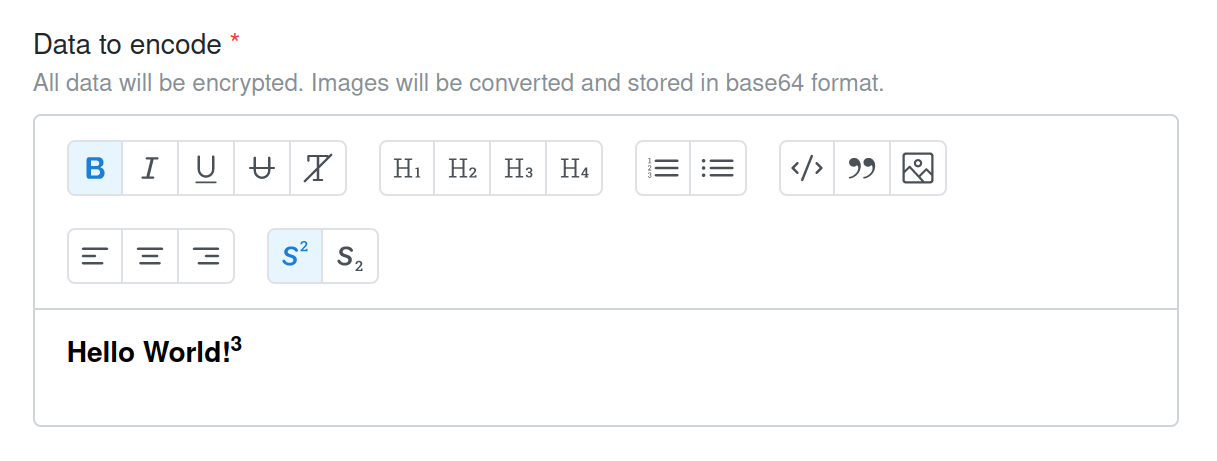
\includegraphics[scale=0.5]{assets/images/encode-editor}
    \caption{Editor textu pro data k zakódování}\label{fig:editor-textu}
\end{figure}

\end{subsubsection}

\begin{subsubsection}{Konfigurace}\label{subsubsec:enc-konfigurace}

Konfigurace je dostupná pouze pro přihlášené uživatele.

V sekci \texttt{Advanced Configuration} je dostupné nastavení parametrů
pro zakódování.

\begin{enumerate}
    \item Vlastní klíč pro zašifrování dat
    \item Počet nejméně významných bitů, které mají být použity
    \item Určení jaké barevné složky mají být změněny
    \item Zda-li mají být data rozprostřena po obrázku rovnoměrně
\end{enumerate}

\end{subsubsection}

\begin{figure}
    \centering
    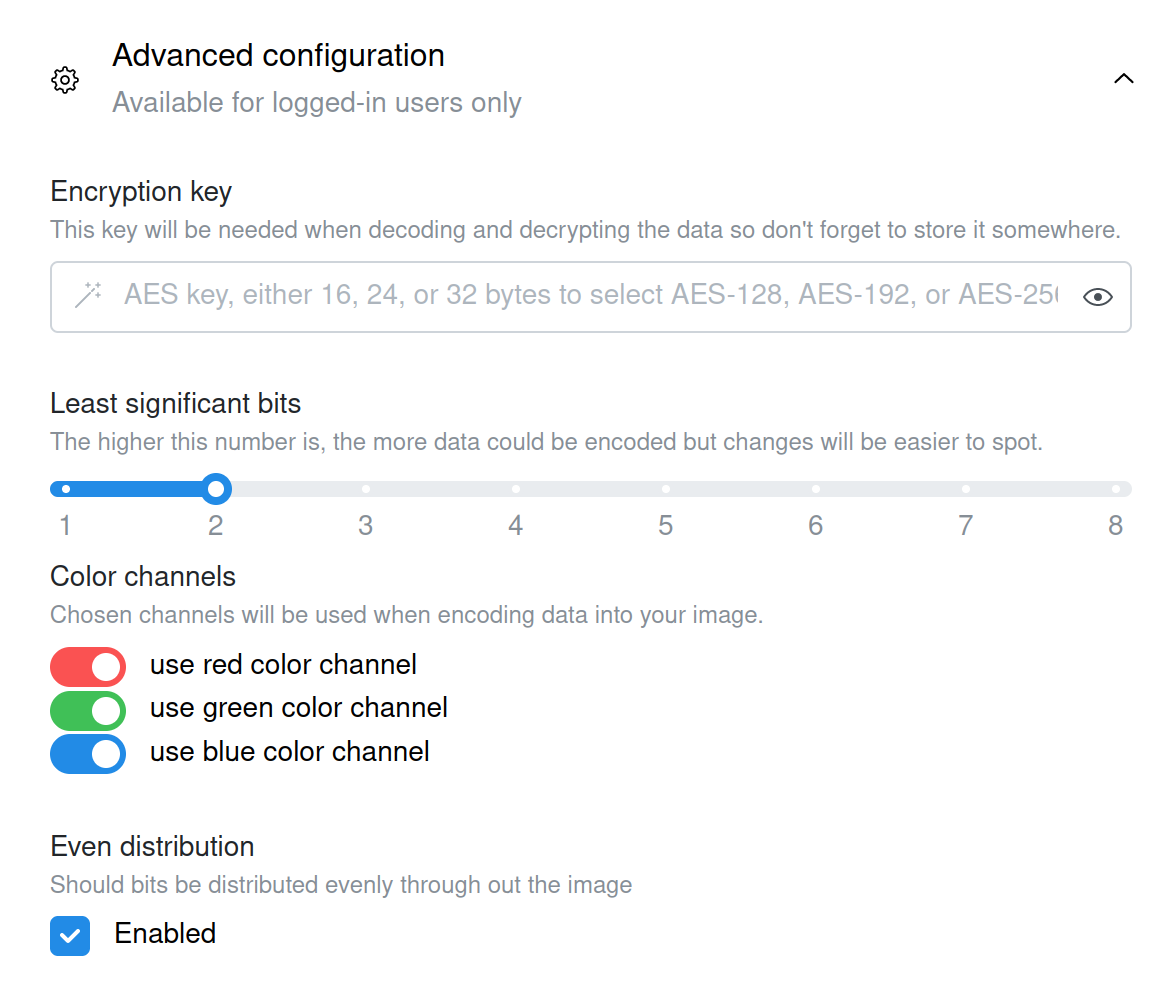
\includegraphics[scale=0.5]{assets/images/encode-configuration}
    \caption{Konfigurace zakódování}\label{fig:konfigurace-zakodovani}
\end{figure}

\begin{subsubsection}{Nahrání obrázku}\label{subsubsec:enc-nahrani-obrazku}

Na stránce nalezneme pole, do kterého lze nahrát obrázek.
Do něj budou informace zakódovány.

\end{subsubsection}

\begin{subsubsection}{Potvrzení}\label{subsubsec:enc-potvrzeni}

Po stisknutí tlačítka \texttt{Encode} proběhne kontrola vložených hodnot.
Pokud je nějaký problém nalezen, aplikace uživatele upozorní.

Dále aplikace pošle požadavek s informací, konfigurací a
obrázkem na server.

Následně server zprávu zašifruje a rozdělí na jednotlivé bity a zapíše je do
obrázku.

Pokud vše proběhne v pořádku, klient dostane zpět odpověď s tímto upraveným
obrázkem.

Dále se uživateli nabídne možnost si obrázek stáhnout.

\end{subsubsection}

\subsection{Dekódování}\label{subsec:dekodovani-dat}
Na adrese \url{https://stegoer.netlify.app/decode} může uživatel nahrát svůj
obrázek a dekódovat z něj data, která tam v minulosti zakódoval.

\begin{subsubsection}{Konfigurace}\label{subsubsec:dec-konfigurace}

V sekci \texttt{Advanced Configuration}, která je opět dostupná pouze
přihlášeným uživatelům, je možné specifikovat vlastní klíč, který má být použit
k odšifrování zprávy.

\end{subsubsection}

\begin{subsubsection}{Nahrání obrázku}\label{subsubsec:dec-nahrani-obrazku}

Na stránce opět nalezneme pole do kterého lze nahrát obrázek.
Z tohotu obrázku se aplikace pokusí zakódovanou informaci dekódovat.

\end{subsubsection}

\begin{subsubsection}{Potvrzení}\label{subsubsec:dec-potvrzeni}

Po stisknutí tlačítka \texttt{Decode} proběhne kontrola vložených hodnot.
Pokud je vše v pořádku, aplikace pošle požadavek s obrázkem a konfiguraci na
server.

Následně server obrázek zpracuje a pokusí se zakódovanou informaci odšifrovat.
Pokud vše proběhne v pořádku, klient dostane zpět odpověd s odšifrovanou
informací.

Na konci stránky se pak tato informace zobrazí.
Aplikace také informaci uživateli zkopíruje do schránky, aby s ní mohl dále
pracovat.

\end{subsubsection}
